\chapter{泥岩流变本构模型及参数拟合}

\todoiZN{这一章要重新梳理,不然查重过不了}
\label{chap:theory}
岩石流变本构模型的建立一直是岩石流变力学理论研究的重点和难点,
合适的本构模型能够较为准确地描述岩石的本质特征,并能较为准确地反映岩石的力学特性和变形机理。因为岩石材料种类繁多,所以流变规律和流变本构模型的表现形式应是多样的,要找到一种普遍适用的、能够全面反映岩石流变力学特性及变形机理的本构模型基本是不可能的。因此,针对工程的实际情况建立适用于该工程本身的本构模型具有重要的意义。目前,建立岩石流变本构模型的方法主要有经验模型、元件模型以及根据热力学内时理论、损伤断裂力学等理论建立岩石的流变本构模型。

\section{流变本构模型}

\subsection{经验模型}
岩石经验流变模型是在岩石流变试验的基础上,通过假设——实验——理论的方法来建立岩石的应力、应变和时间的函数关系模型。经验型蠕变本构模型往往采用幂函数、对数函数、指数函数、双曲线函数等数学表达式。此类模型虽然较为直观,应用方便,但其只是通过流变表观现象获得,物理意义不明确,只适合描述在特定试验条件下的流变行为。

岩石的典型蠕变曲线是通过大量的岩石单轴压缩蠕变试验,在恒定应力水平 作用下,总结出来的岩石随时间的变形规律,其蠕变方程可表示为:
\begin{equation}
     {\varepsilon}={\varepsilon}_{0}+{\varepsilon}_{1}+{\varepsilon}_{2}+{\varepsilon}_{3}
\end{equation}

式中,$\varepsilon$为总应变,$\varepsilon_0$为瞬时应变,$\varepsilon_1$、$\varepsilon_2$、$\varepsilon_3$分别为衰减蠕变阶段、等速蠕变阶段和加速蠕变阶段的应变。

\begin{figure}[ht!]
    \centering
            \centering
            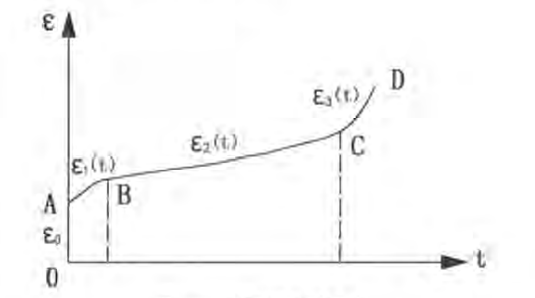
\includegraphics[width=0.5\textwidth]{img/chap3/蠕变曲线.png}
    \caption{蠕变曲线}
    \label{fig:3-1}

\end{figure}

由于岩石加速蠕变阶段变形规律复杂而且持续时间极为短暂,大多数经验模型都只是对岩石第一、第二阶段的蠕变变形进行描述,常见的蠕变经验公式如下:

1)幂函数型
\begin{equation}
     {\varepsilon}(t)=At^n
\end{equation}
式中,$A$、$n$是材料常数,其值与应力水平、材料特性和温度条件相关,多用于
反应减速蠕变阶段的性质。

2)对数型
\begin{equation}
     {\varepsilon}(t)={\varepsilon}_{0}+Blgt+Dt
\end{equation}
式中,$B$、$D$为与应力有关的常数,常用于反应加速蠕变阶段的性质。

3)指数型
\begin{equation}
     {\varepsilon}(t)=A[1-exp(f(t))]
\end{equation}
式中,$A$为材料常数、f(t)为时间f的函数,多用于反应等速蠕变阶段的性质。


上述经验流变本构模型是根据试验结果抽象得到的应力-应变—时间关系,不同的岩石,甚至相同岩石的不同试验都会得出不同的经验公式,因此必须在特定条件下才能得出相应的经验流变模型中。在建立模型时,主要运用以下三种蠕变技术理论:

(1)老化理论

老化理论的流变状态方程以应变、应力和时间之间的关系来表示:
\begin{equation}
     {\varepsilon}=f({\sigma},{t})
\end{equation}

根据维亚络夫在《土力学的流变原理》中介绍的老化理论,总应变被视作瞬时弹性应变和蠕变应变的和,假设瞬时弹性应变为$\varepsilon_0$,蠕变应变为$\varepsilon_c$,则应变方程可表示为:
\begin{equation}
     {\varepsilon}={\varepsilon_0}+{\varepsilon_c}
\end{equation}
假设取$\varepsilon_c$=$\frac{\sigma}{E}$,$\varepsilon_e$=$f(\sigma){\Phi}'(t)$,式(2.6)可得:
\begin{equation}
     {\varepsilon}={\varepsilon_0}+{\varepsilon_c}=\frac{\sigma}{E}+f(\sigma){\Phi}'(t)
\end{equation}
函数币${\Phi}'(t)$表征了变形的增长随时间而减缓,从本质上反映了材料特性随时间的变化即“老化”,老化理论适用于确定某个具体时刻的变形值,而不依赖于这一时刻前的受荷历史,即不研究变形的全过程。当应力历史较为复杂时并不适用。

(2)流动理论

流动理论的流变状态方程以应变速率、应力和时间之间的关系来表示,变形速率等于弹性变形速率加蠕变变形速率:
\begin{equation}
     {\dot{\varepsilon}}=f({\sigma},{t})={\dot{\varepsilon_0}}+{\dot{\varepsilon_c}}
\end{equation}
假设$\dot{\varepsilon_0}$=$\frac{1}{E}\frac{\mathrm{d} \sigma}{\mathrm{d} t}
$,$\dot{\varepsilon_c}$=$f(\sigma)\chi(t)$,
\begin{equation}
     {\dot{\varepsilon}}=\frac{1}{E}\frac{\mathrm{d} \sigma}{\mathrm{d} t}+f(\sigma)\chi(t)
\end{equation}
“流动理论”这一名称是根据这个理论的方程和粘滞流动方程相似而得到的。蠕变方程通过对式(2.9)进行求积分得方式获得。

(3)硬化理论

硬化理论建立的是以应变速率、应力和应变本身所构成的表达式:
\begin{equation}
     {\dot{\varepsilon}}=f({\sigma},{\varepsilon})=\frac{f(\sigma)}{\phi(\varepsilon)}
\end{equation}

从这个式子可看出应变速率随应变的增加而减小,物体仿佛硬化了,这个理论因此而得名。

\subsection{元件组合模型}
元件组合模型是考虑岩体种类、应力、温度、湿度、辐射等因素的影响,表现出的一系列与时间相关的力学响应。以三种基本元件——弹性元件、粘性元件及塑性元件以不同的形式串联或并联组合成为某种更复杂的模型,据此推导其本构方程来近似地建立所研究岩石的本构关系。而对于特定的影响条件,如温度、湿度等,则通过该使用不同特性的基本元件来表示。目前学者们提出的模型有很多种,现在常见的模型有Burgers模型、西原模型和H-K模型等。下面介绍几种基本元件及简单的组合模型。

1.基本元件的力学模型

(1)弹性元件
\begin{figure}[ht!]
    \centering
            \centering
            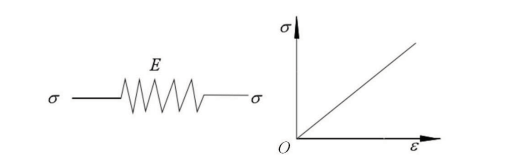
\includegraphics[width=0.6\textwidth]{img/chap3/Elastic element.png}
    \caption{弹性元件}
    \label{fig:3-2}
\end{figure}

弹性元件可以用弹簧表示,其应力-应变为线性关系,如图~\ref{fig:3-2},满足胡克定律,又称为胡克体(H),一维状态下的本构方程为:

\begin{equation}
{\sigma}={E}{\varepsilon}
\end{equation}

弹性元件的应力-应变关系不随时间变化,其应变是瞬时完成的,因此其不具有蠕变和松弛等流变特性。

(2)粘性元件
\begin{figure}[ht!]
    \centering
            \centering
            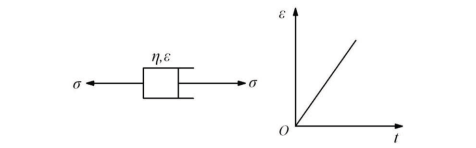
\includegraphics[width=0.6\textwidth]{img/chap3/Viscous element.png}
    \caption{粘性元件}
    \label{fig:3-3}
\end{figure}

粘性元件用于模拟材料的粘滞性,用粘壶表示,理想粘性体的应变与时间成线性关系,可称之为牛顿体(N),如图~\ref{fig:3-3}。可以认为粘壶是一个带孔的活塞在充满牛顿液体的圆筒
中运动。$\eta$为粘滞系数,表示应力与应变速率的比值,在一维状态下其本构方程为:

\begin{equation}
{\sigma}={\eta}\overset{\centerdot }{\mathop{\boldsymbol{\varepsilon}}}
\end{equation}

粘性元件在受力后不立即产生应变,应变随着时间的发展逐渐增大,具有流变特性。在受力过程中移去应力,应变不会恢复。

(3)塑性元件
\begin{figure}[ht!]
    \centering
            \centering
            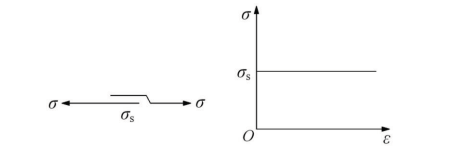
\includegraphics[width=0.6\textwidth]{img/chap3/Plastic element.png}
    \caption{塑性元件}
    \label{fig:3-4}
\end{figure}

塑性元件用于模拟材料的塑性,由一对接触面粗糙的滑块组成,如图~\ref{fig:3-4},又称圣维南塑性体(S),其在一维状态下其本构方程为:

\begin{equation}
    \left\{\begin{matrix}
               \varepsilon =0& \sigma <{{\sigma }_{s}} & \\
               \varepsilon \to \infty & \sigma \ge {{\sigma }_{s}}  &
    \end{matrix}\right.
\end{equation}

当塑性体应力小于材料的屈服极限时,塑性体表现出刚体的性质,不产生任何变形,而当其应力达到或超过屈服极限时,可产生任意应变值,并且即使应力不再增加,应变也会持续增长,一旦应力去除,应变增长停止而留下永久变形。

通过将以上三种基本元件进行串并联组合可以清晰地反映岩石的黏弹性、黏塑性和
黏弹塑性等流变性质。

2.组合模型

(1)Maxwell(马克斯威尔)模型

该模型时由一个弹性元件和一个粘性元件串联形成得粘弹性体。
\begin{figure}[ht!]
    \centering
            \centering
            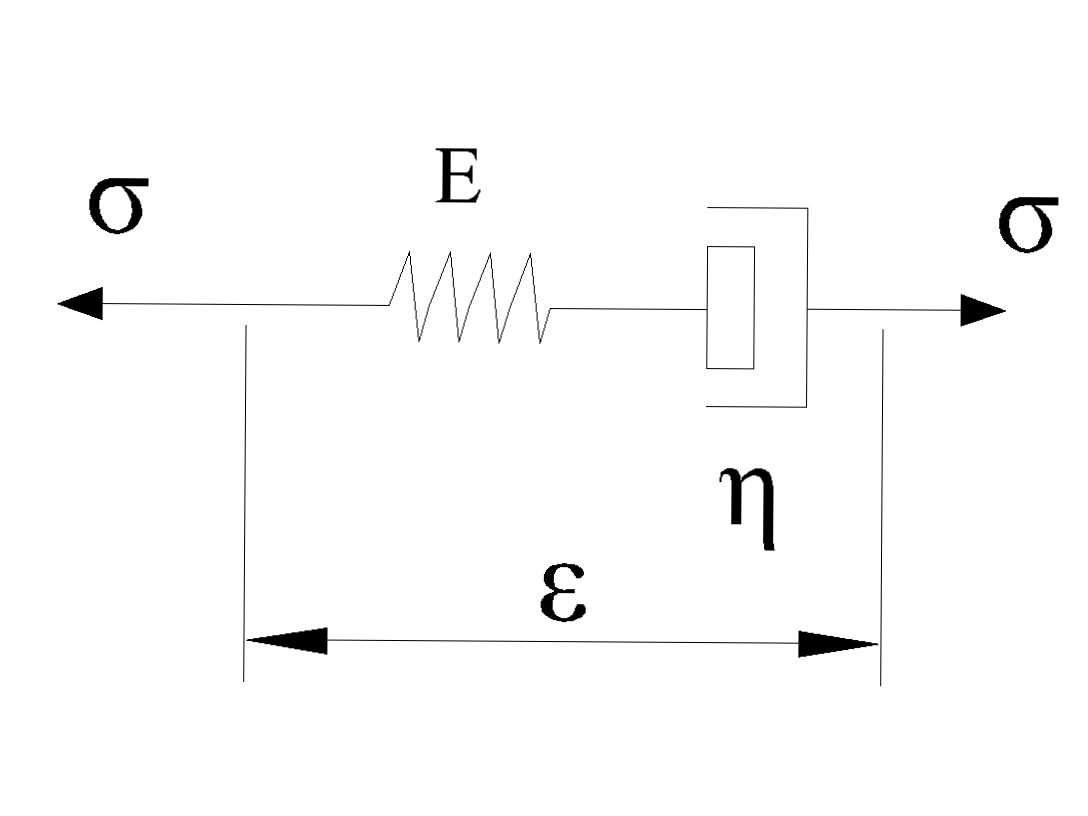
\includegraphics[width=0.4\textwidth]{img/chap3/Maxwell.png}
    \caption{Maxwell模型}
    \label{fig:3-5}
\end{figure}

由两个元件串联可得:
\begin{equation}
\left\{\begin{matrix}
          &\sigma ={{\sigma}_{1}}={{\sigma }_{2}}   \\
          &\boldsymbol{\varepsilon} ={{\boldsymbol{\varepsilon} }_{1}}+{{\boldsymbol{\varepsilon} }_{2}} 
         =\frac{{\sigma }_{1}}{E}+\frac{{\sigma }_{2}}{\eta}
        \end{matrix}  
 \right.
\end{equation}

由上式可模型本构方程为:
\begin{equation}
     \overset{\centerdot }{\mathop{\boldsymbol{\varepsilon} }}\,=\frac{1}{E}\overset{\centerdot }{\mathop{\sigma }}\,+\frac{1}{\eta }\overset{\centerdot }{\mathop{\sigma }}
\end{equation}

施加恒定应力$\sigma_0$,此时Maxwell模型的蠕变方程为:
\begin{equation}
     {\varepsilon}=\frac{\sigma_0}{E}+\frac{\sigma_0}{\eta }t
\end{equation}


2.Kelvin(开尔文)模型

该模型由一个弹性元件与一个粘性元件并联而成。
\begin{figure}[ht!]
    \centering
            \centering
            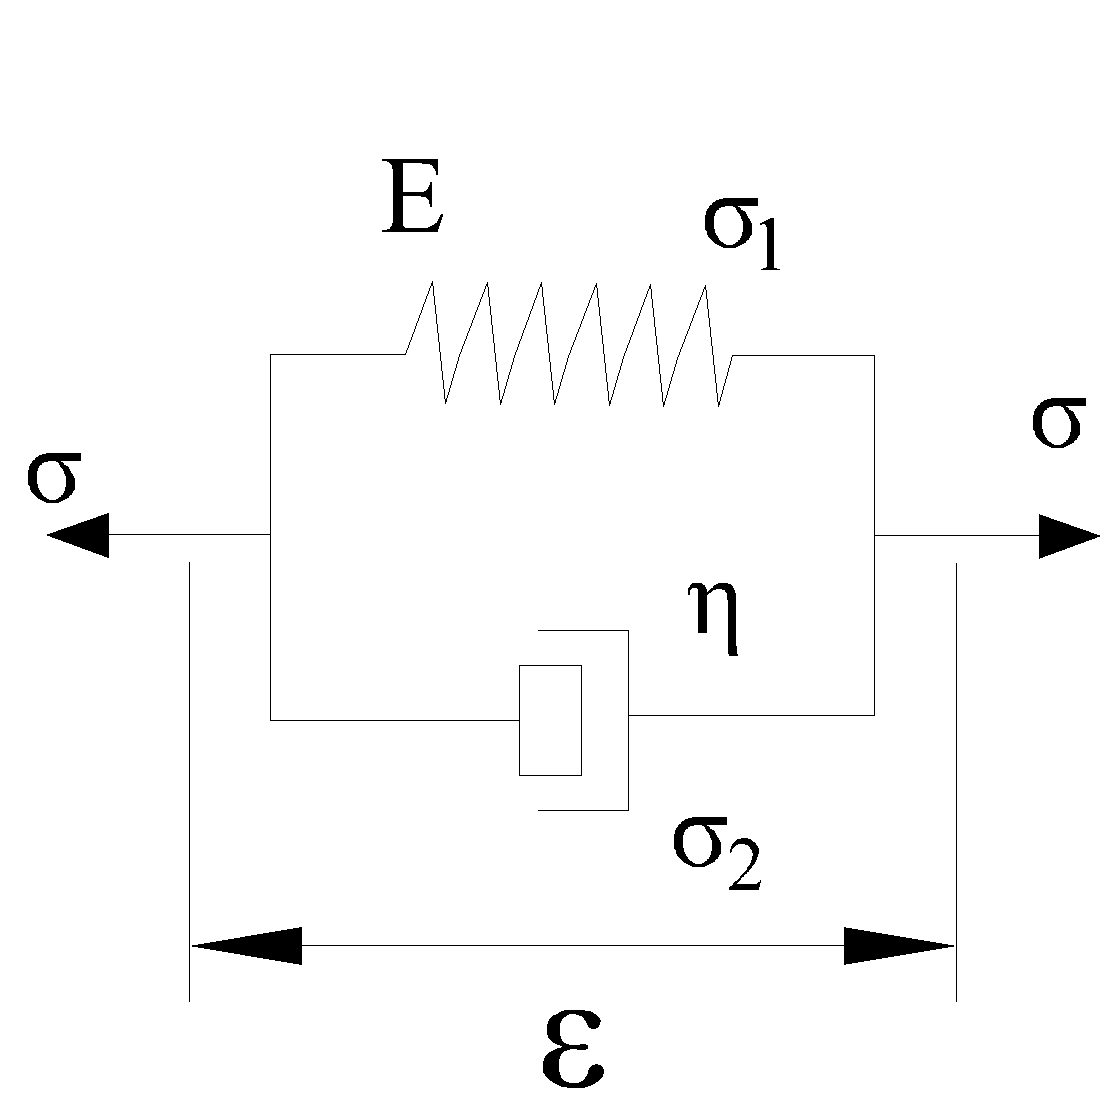
\includegraphics[width=0.4\textwidth]{img/chap3/Kelvin.png}
    \caption{Kelvin模型}
    \label{fig:3-6}
\end{figure}

由两个元件并联可得如下方程组:

\begin{equation}
  \left\{
  \begin{matrix}
 &\sigma =\sigma _1+\sigma _2  \\
 & \boldsymbol{\varepsilon} =\boldsymbol{\varepsilon}_1=\boldsymbol{\varepsilon}_2\\ 
 & \sigma _1=E \boldsymbol{\varepsilon}_1  \\
 & \sigma _2=\eta \dot{\boldsymbol{\varepsilon}_2}
 \end{matrix}
 \right.
\end{equation}

由式(3.11)可求得Kelvin模型得本构方程为:
\begin{equation}
\sigma=E\boldsymbol{\varepsilon}+\eta\dot{\boldsymbol{\varepsilon}}
\end{equation}

施加恒定应力$\sigma_0$,此时Kelvin模型的蠕变方程为:
\begin{equation}
     {\varepsilon}=\frac{\sigma_0}{E}(1-e^{-\frac{E}{\eta }t})
\end{equation}


3.粘塑性模型

该模型由一个粘性元件和一个塑性元件并联组成,用来模拟材料的粘塑性,如下图~\ref{fig:3-7}所示,用符号表示为V|N。粘塑性模型在应力加载时不产生弹性应变,因此在应力卸载后,模型发生的变形不能恢复。

\begin{figure}[ht!]
    \centering
            \centering
            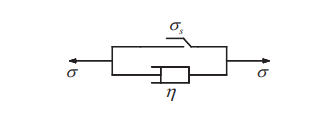
\includegraphics[width=0.4\textwidth]{img/chap3/V-N.png}
    \caption{粘塑性模型}
    \label{fig:3-7}
\end{figure}

当$\sigma$小于岩石材料屈服极限$\sigma_s$时,塑性元件不起作用,整体应变$\varepsilon$=0;当$\sigma$ $\geq$ $\sigma_s$时,塑性元件开始工作,模型产生粘塑性变形,由此可得该模型的本构方程为:

\begin{equation}
    \left\{\begin{matrix}
               \boldsymbol{\varepsilon} =0& \sigma <{{\sigma }_{s}} & \\
               \overset{\centerdot }{\mathop{\boldsymbol{\varepsilon} }}\,=\frac{\sigma -{{\sigma }_{s}}}{\eta } & \sigma \ge {{\sigma }_{s}}  &
    \end{matrix}\right.
\end{equation}

施加恒定应力$\sigma_0$后,该模型的蠕变方程为:
\begin{equation}
    \left\{\begin{matrix}
               \boldsymbol{\varepsilon} =0& \sigma <{{\sigma }_{s}} & \\
               {\varepsilon}=\frac{\sigma -{{\sigma }_{s}}}{\eta }t & \sigma \ge {{\sigma }_{s}}  &
    \end{matrix}\right.
\end{equation}

组合模型能够较好反应岩石流变各个阶段的变形特性,将基本元件相互组合可以得到具有粘弹、粘塑和粘弹塑性的本构模型。在一维状态下,目前较常用的线性流变组合模型如下表所示:
\begin{table}[ht!]\small
    \begin{tabular}{ccc}
    \toprule
        \makebox[0.1\textwidth][c]{模型名称} & \makebox[0.2\textwidth][c]{模型组成} & \makebox[0.4\textwidth][c]{本构方程}  \\
        \midrule
        \rule{0pt}{15pt}
        广义Kelvin模型        & H-(H|N)  &   \normalsize{$\sigma+\frac{\eta_1}{E_1+E_2}\dot{\sigma}=\frac{{E_1}{E_2}}{E_1+E_2}\varepsilon+\frac{{E_1}{\eta_1}}{E_1+E_2}\dot{\varepsilon}$}   \\ 
        \rule{0pt}{50pt}
        西原模型              & H-(H|N)-(S|N)  &  \normalsize{\makecell[c]{$\sigma \textless \sigma_s$,\\$\sigma+\frac{\eta_1}{E_1+E_2}\dot{\sigma}=\frac{{E_1}{E_2}}{E_1+E_2}\varepsilon+\frac{{E_1}{\eta_1}}{E_1+E_2}\dot{\varepsilon}$\\
        $\sigma \textgreater \sigma_s$,\\
        $(\sigma-\sigma_s)+(\frac{\eta_2}{E_1}+\frac{\eta_1+\eta_2}{E_2})\dot{\sigma}+\frac{\eta_1\eta_2}{E_1E_2}\ddot{\sigma}={\eta_2}{\dot{\varepsilon}}+\frac{\eta_1\eta_2}{E_1}\Ddot{\varepsilon}$}}\\
        \rule{0pt}{30pt}
        Burgers模型    &    H-N-(H|N)    &  \normalsize{$\sigma+(\frac{\eta_1}{E_1}+\frac{\eta_1+\eta_2}{E_2})\dot{\sigma}+\frac{\eta_1\eta_2}{E_1E_2}\ddot{\sigma}={\eta_1}{\dot{\varepsilon}}+\frac{\eta_1\eta_2}{E_2}\Ddot{\varepsilon}$}\\
        \rule{0pt}{30pt}
        广义Bingham模型  &   H-(N|S)  &  \normalsize{\makecell[c]{$\sigma \textless \sigma_s$,$\varepsilon=0$   \\
        $\sigma \textgreater \sigma_s$,$\dot{\varepsilon}=\frac{\dot{\sigma}}{E}+\frac{\sigma-\sigma_s}{\eta}$}}\\
    \bottomrule
        
    \end{tabular}
    \caption{常用组合模型及其本构方程}
    \label{tab:常用组合模型及其本构方程}
\end{table}

\section{岩石线性流变模型及参数拟合}
根据试验结果总结泥岩流变曲线的特征可以发现,在加载应力后会出现瞬时弹性变形,再之后会有随时间增长的流变变形,因此本构模型应该包含弹性元件和粘性元件。在进入稳定蠕变阶段后,蠕变速率减小到接近于0,因此可以用Kelvin模型来描述泥岩的衰减蠕变阶段。本文在这里选用经典Burgers模型来描述泥岩的线性流变力学特性。

burgers模型是由一个Maxwell体和一个Kelvin体串联构成的,具体形式如图所示:
\begin{figure}[ht!]
    \centering
            \centering
            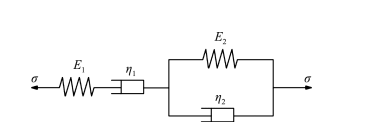
\includegraphics[width=0.6\textwidth]{img/chap3/Burgers.png}
    \caption{Burgers模型}
    \label{fig:3-8}
\end{figure}
Burgers模型的总应力和总应变可以表示为:
\begin{equation}
    \left\{\begin{matrix}
               \sigma=\sigma_1=\sigma_2  \\
               \varepsilon = \varepsilon_1+\varepsilon_2\\
    \end{matrix}\right.
    \label{eq:3-22}
\end{equation}

\begin{figure}[ht!]
    \centering
            \centering
            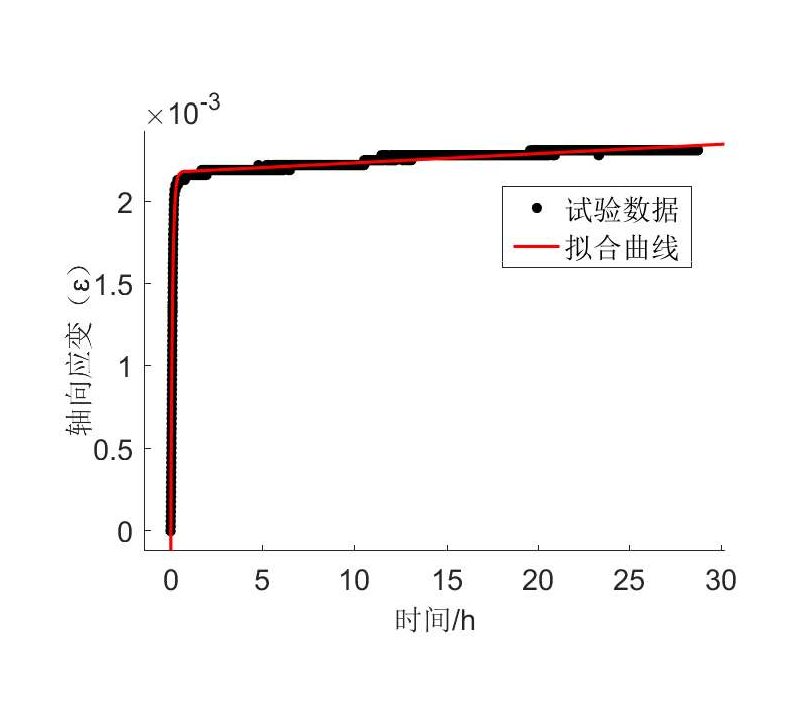
\includegraphics[width=0.7\textwidth]{img/chap3/C-01.pdf}
    \caption{Burgers模型}
    \label{fig:3-9}
\end{figure}




由于Burgers模型是由Maxwell体和Kelvin体串联而成,根据他们的本构方程和串联元件的应力和应变关系(如式\ref{eq:3-22}),消去$\varepsilon_1$和$\varepsilon_2$,可以求得Burgers模型的本构方程为:
\begin{equation}
    \sigma+(\frac{\eta_1}{E_1}+\frac{\eta_1+\eta_2}{E_2})\dot{\sigma}+\frac{\eta_1\eta_2}{E_1E_2}\ddot{\sigma}={\eta_1}{\dot{\varepsilon}}+\frac{\eta_1\eta_2}{E_2}\Ddot{\varepsilon}
    \label{eq:3-23}
\end{equation}

在流变试验中,当荷载恒定时,令$\sigma=\sigma_0$,代入式\ref{eq:3-23}整理得到Burgers模型的流变方程为:
\begin{equation}
    \varepsilon(t)=\frac{\sigma_0}{E_1}[1-exp(-\frac{E_1}{\eta_1}t)]+\frac{\sigma_0}{E_2}+\frac{\sigma_0}{\eta_2}t
    \label{eq:3-23}
\end{equation}


\section{岩石非线性流变模型及参数拟合}
\subsection{泥岩非线性流变模型确定}
大量的试验研究结果表明,泥岩具有非线性流变特征,而这种特征在加速流变阶段最为明显,为了更确切地描述泥岩的流变特性,就要研究岩石的非线性流变问题,目前构建岩石非线性流变模型的方法有:

(1)基于实验结果,通过回归分析拟合经验方程,针对岩石流变的非线性问题,可以采用幂函数型的经验公式:
\begin{equation}
     {\dot\varepsilon}=A\sigma^nt^m
\end{equation}

$\dot\varepsilon$为流变速率,$\sigma$为加载应力水平,$t$为加载时间,A,n,m为与材料、应力、时间相关的参数,可以根据流变实验结果拟合得到。

(2)基于现有的线性流变模型,串联或并联一个非线性元件,构建一个可以描述流变加速阶段的流变本构模型。

(3)把线性元件组合模型中的线性元件替换为非线性元件,或将模型中的线性元件参数改为与材料、应力、时间相关的非常定参数方程,以此来研究岩石的非线性流变问题。

(4)结合内时理论、损伤断裂力学等理论等方法,在线性流变模型中引入损伤变量,达到构建非线性流变模型的目的。

本文拟采用第一种方法,利用试验数据对经验公式进行拟合得到泥岩的非线性本构模型。根据试验结果,泥岩流变过程受到时间、应力等因素的影响,再考虑到温度对工程中围岩流变的影响,本文拟采用根据Wallner、Hunsche和Schulze等基于错位理论,从盐岩细观结构层面提出的BGRa流变本构模型进行模拟研究\cite{1981Thermomechanical,Hunsche1999Rock},该模型是一种幂函数型的本构模型。他们认为盐岩是一种多晶材料,其蠕变行为在本质上是晶体错位运动的结果。岩盐的初始瞬态蠕变阶段仅持续时间较短。且初始蠕变量在总蠕变量中所占比例很小。因此在不考虑初始蠕变与加速蠕变阶段的情况下,可采用稳态蠕变模型研究长期变形,这也符合流变试验所得出的结论。

引入BGRa模型来描述泥岩稳态流变变形随温度和应力的函数关系:

\begin{equation}
    \dot{\boldsymbol{\varepsilon}}=A\mathrm{exp}\left ( -\frac{Q}{RT}\right ) \left (\frac{\sigma_1-\sigma_3}{\sigma^*}\right )^m
\end{equation}
\begin{shizhong}
    \item $A$、$n$\,---\,为材料参数;
    \item $Q$\,---\,为材料的有效激活能;
    \item $R$\,---\,为理想气体常数;
    \item $T$\,---\,试验温度;
\end{shizhong}

在BGRa模型中,将蠕变速率描述为:
\begin{equation}
    \begin{gathered}
        \dot { \boldsymbol{\varepsilon}}^\text{cr} ({ \boldsymbol{\sigma}})={\color{black} {\sqrt{\frac{3}{2}}}}Ae^{-Q/(RT)}\left(\dfrac{{\bar \sigma}}{\sigma_\text{ref}}\right)^m\dfrac{{\boldsymbol s}}{{\left\Vert{\boldsymbol s}\right\Vert}}
    \end{gathered}
\end{equation}

其中, ${ \bar\sigma}$ 为等效应力, ${ \bar\sigma}={\sqrt{{\frac{3}{2}}}}{\left\Vert{\boldsymbol s}\right\Vert}$ ,偏应力 ${\boldsymbol s}= { \boldsymbol{ \sigma}}-\frac{1}{3}{ \mathrm{tr}(\boldsymbol{\sigma}}){\mathbf I}$.

通过引入:
\begin{equation}
    b={\left(\dfrac{3}{2}\right)^{(m+1)/2}} \dfrac{Ae^{-Q/(RT)}}{\sigma_\text{ref}^m}
\end{equation}

即蠕变应变率可表示为:
\begin{equation}
    \begin{gathered}
        \dot { \boldsymbol{\varepsilon}}^\text{cr} ({ \sigma}) = b {\left\Vert{\boldsymbol s}\right\Vert}^{m-1} {\boldsymbol s}
    \end{gathered}
    \label{eq:bgra}
\end{equation}

最终,考虑蠕变和热应变的总应变率可表示为:
\begin{equation}
    \begin{gathered}
        \dot { \boldsymbol{\varepsilon} }= \dot { \boldsymbol{\varepsilon}}^\text{el} + \dot {\boldsymbol{\varepsilon}}^\text{th}
        + \dot { \boldsymbol{\varepsilon}}^\text{cr}
    \end{gathered}
\end{equation}
其中, $\dot {\boldsymbol{\varepsilon}}^\text{el}$ 是弹性应变率, $\dot { \boldsymbol{\varepsilon}}^\text{th}$ 是热应变率,  $\dot {\boldsymbol{\varepsilon}}^\text{cr}$是蠕变应变率。


\subsection{非线性流变模型参数辨识}
常见的参数识别方法有最小二乘法,最小二乘法的基本原理为根据n组试验数据$(X_k,Y_k)(k=1,2,3,\dots,n)$,应变量Y是自变量X和待求参数A的确定函数,$Y=f(X,A)$,其中自变量X和待求参数A可以有多个$(X=\{x_1,x_2,…,x_p\},A=\{a_1,a_2,…,a_q\})$。要求出参数$a$,就要使残差平方和Q达到最小值,必须满足如下条件:
\begin{equation}
    Q=\sum_{k=1}^n[Y_k-f(X_k,A)]^2
\end{equation}

\begin{equation}
    \frac{\partial{Q}}{\partial{a_i}}=0(i=1,2,\dots,q)
\end{equation}

Levenberg-Marquardt非线性优化最小二乘法,即$L-M$算法,是一种介于牛顿法和梯度下降法之间的非线性优化算法。对于过参数化的问题不敏感,能有效处理冗余参数的问题,使代价函数陷入局部极小值的机会大大
减小,这些特性使得$L-M$算法在各领域都得到广泛应用。L-M算法本质上是在迭代过
程中把原问题化为多个$LS$问题进行求解。其非线性关系的一般形式为:
\begin{equation}
    y=f(x,d)
\end{equation}

其中f为给定的非线性函数;$x=(x_1,x_2,\dots,x_m))$为自变量向量,$d=(d_1,d_2,\dots,d_n)$为未知参数向量,假设对x和y进行p次运算,得到p组数据X和Y,其残差平方和e为:
\begin{equation}
    e=\sum_{i=1}^p[Y_i-f(X_i,d)]^2
\end{equation}

$L-M$算法的目的是求出一组d使e极小化。若第k次迭代结果为$d^(k)$,则将f(X,d)在$d^(k)$附
近的一阶近似表示为:
\begin{equation}
    f(d^{(k)}+\delta^{(k)})\approx f(x,d^{(k)})+A^{(k)}\delta^{(k)}
\end{equation}

其中:
\begin{equation}
    A^{(k)}=[\frac{\partial{f(x,d)}}{\partial{d_j}}]_{d=d^{(k)}},j=1,2,\dots,n
\end{equation}

使得:
\begin{equation}
    {\left\Vert{\boldsymbol y-f(x,b^{(k+1)})}\right\Vert}=\mathop{\min}_{\delta^k}{\left\Vert{\boldsymbol A^{(k)}\delta^{(k)}-e^{(k)}}\right\Vert}
\end{equation}

也就是在己知$A^{(k)}$和$e^{(k)}$的情况下,解超定线性方程$A^{(k)}\delta^{(k)}=e^{(k)}$,其最小二乘解为:

\begin{equation}
    \label{eq:3-35}
    (\delta^{(k)})_{LS}=((A^{(k)})^{'}A^{(k)})^{-1}(A^{(k)})^{'}e^{(k)}
\end{equation}

而对于L-M算法,用$(A^{(k)})^{'}A^{(k)}+{\lambda_k}I$代替式\ref{eq:3-35}中的$(A^{(k)})^{'}A^{(k)}$,则有:

\begin{equation}
    (\delta^{(k)})_{LM}=((A^{(k)})^{'}A^{(k)}+{\lambda_k}I)^{-1}(A^{(k)})^{'}e^{(k)}
\end{equation}

其中:$\lambda_k$和${\lambda_k}I$分别称为阻尼因子和阻尼项,这使得L-M算法相较于最小二乘法,克服了系数矩阵奇异和病态时导致的异常情况。当$\lambda_k$=0时,即为高斯.牛顿法;当$\lambda_k$取值很大时,接近梯度下降法。由于$L-M$算法利用了近似的二阶导数信息,故比梯度下降法快得多。基于以上优点,
本文选择$L-M$算法进行参数拟合。

首先,我们需要考虑的是符合上一章所完成试验的具体情况——在进行流变试验时,未考虑温度因素的影响,所以对BGRa模型进行一定程度的修改:

\begin{equation}
    \dot{\boldsymbol{\varepsilon}}=A\Delta\sigma^m
    \label{eq:3-37}
\end{equation}

$\Delta\sigma$——试验过程中所施加的偏应力

根据泥岩室内流变试验得到的数据,采用Levenberg-Marquardt非线性优化最小二乘法对式\ref{eq:3-37}的位置参数A、m进行拟合。基于Origin软件的非线性曲线拟合功能,自定义拟合函数为变形后的BGRa流变方程。在本次曲线拟合中,我们需要确定的是加载应力水平对流变速率的影响关系,而BGRa模型是描述稳态蠕变阶段的本构模型,因此我们在选择拟合数据时,选择对应各级加载应力水平的稳态蠕变阶段的流变速率。

在拟合数据时,因为在C-03这一组试验中几乎不存在稳定蠕变阶段,试样在应力施加后很快就破坏了,所以单轴流变试验选取了除C-03以外的四组数据。而在三轴流变试验的三组数据中,选取了完整度比较高的D-02的分级加载试验数据,对每一级的应力及稳定蠕变速率的参数方程进行了数据拟合。计算出各试样的蠕变经验模型参数如表\ref{tab:单、三轴试验BGRa流变模型参数}所示,对应的拟合曲线如图\ref{fig:3-8}、\ref{fig:3-9}所示。

\begin{table}[ht!]\small
    \begin{tabular}{p{3cm}<{\centering} p{3cm}<{\centering} p{3cm}<{\centering} p{3cm}<{\centering}}
        \toprule
        试样编号  & $A$  &  $m$   & 拟合效果/$R^2$\\
        \midrule
           C     &   1.14791E-18   &    8.90542   &   0.976\\
        \midrule
        D-02    &   9.61511E-18   &    6.42455   &   0.992 \\
        \bottomrule
    \end{tabular}
    \caption{BGRa流变模型参数}
    \label{tab:单、三轴试验BGRa流变模型参数}
\end{table}

\begin{figure}[ht!]
    \centering
            \centering
            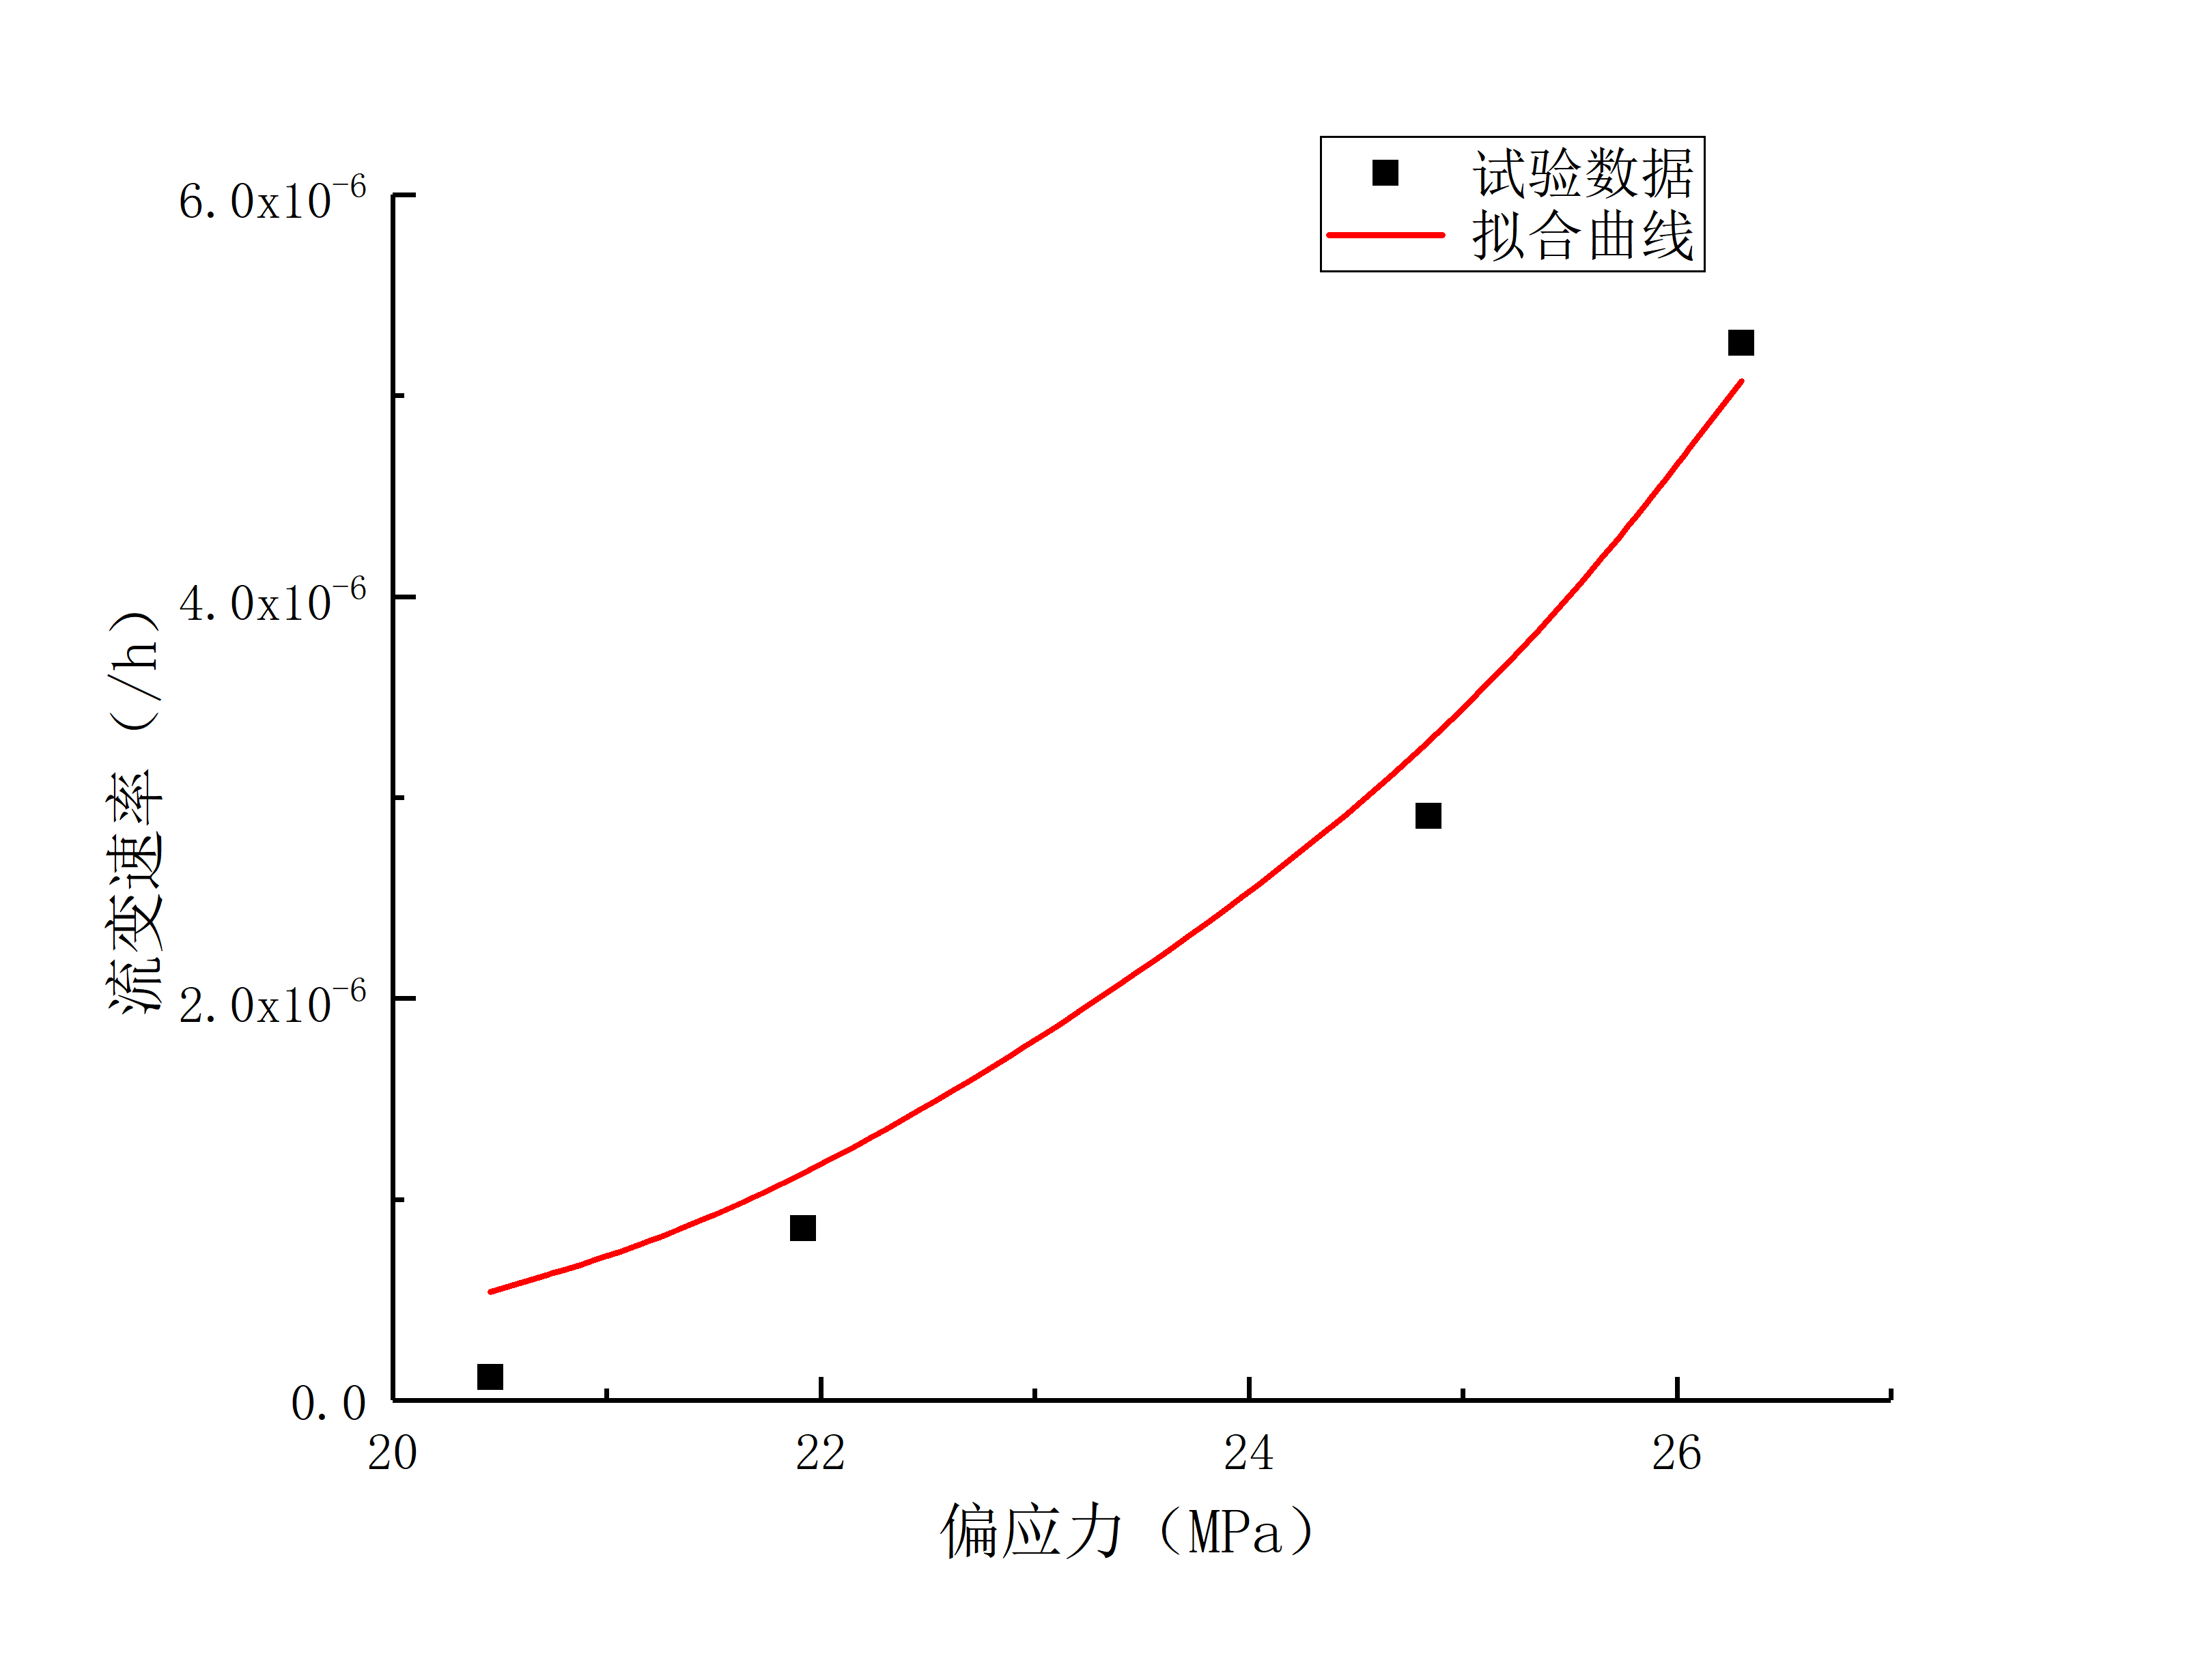
\includegraphics[width=0.6\textwidth]{img/chap3/Uniaxial curve fitting.png}
    \caption{单轴流变速率试验数据和拟合曲线}
    \label{fig:3-8}
\end{figure}

\begin{figure}[ht!]
    \centering
            \centering
            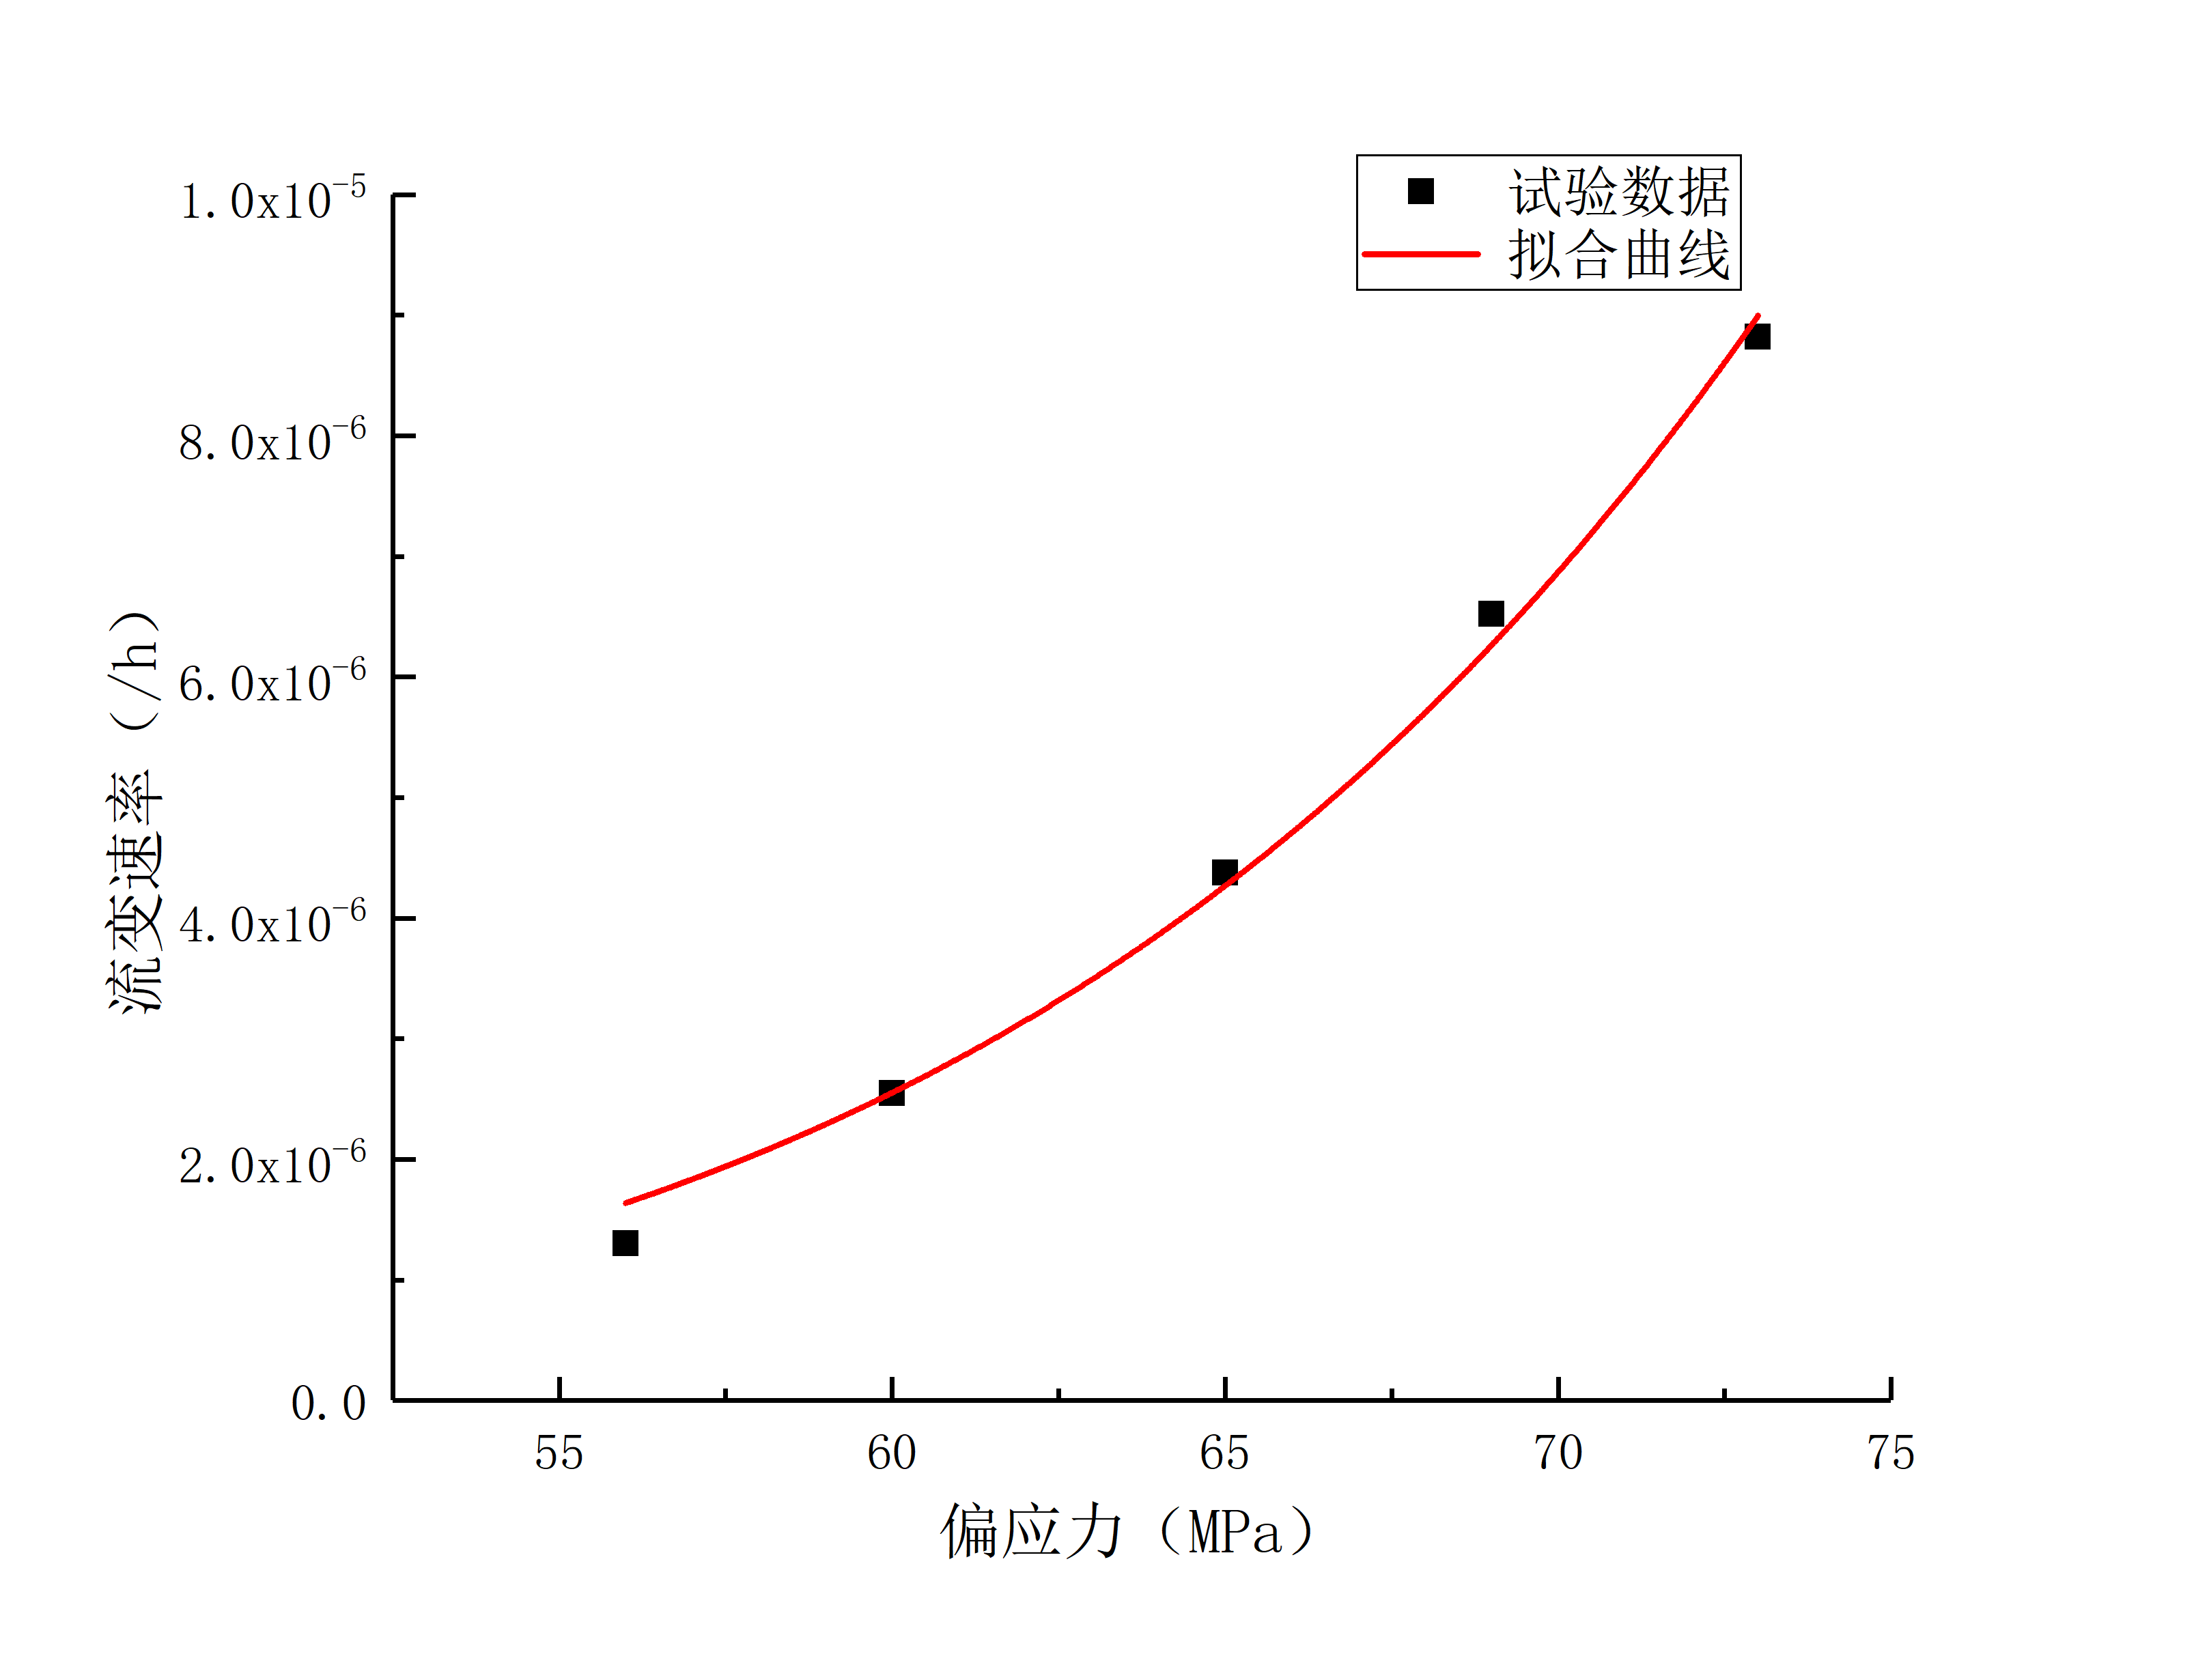
\includegraphics[width=0.6\textwidth]{img/chap3/Triaxial curve fitting.png}
    \caption{10MPa围压下流变速率试验数据和拟合曲线}
    \label{fig:3-9}
\end{figure}

由上述表中的数据和拟合曲线图可以看出,在单轴试验和三轴试验中,泥岩的稳态流变速率都随着加载应力等级的提升而增大。由图\ref{fig:3-8}和\ref{fig:3-9}可知,BGRa流变模型拟合曲线与蠕变试验结果总体吻合较好,但在应力较低的水平下拟合有所偏差。两条曲线拟合平均调整后的$R^2$分别为0.976和0.992,说明整体拟合的效果较好,而且对于三轴试验中的数据拟合效果更好。总体上来说,BGRa流变模型可以用来描述该泥岩的流变特性。

\section{小结}
本章对岩石的线性流变元件和基本流变本构模型进行了简单介绍,选取了xxx和BGRa等不同的本构模型来描述稳态蠕变阶段的泥岩的流变速率的特征,并对该流变方程进行了参数拟合,得到如下主要成果:

(1)经验型流变本构模型往往根据试验结果,不追求岩石的流变机理,通过数学函数抽象得到的应力、应变、时间关系,属积分型本构方程。在本章中简单介绍了常用的幂函数模型、指数模型、对数模型等经验模型,以及在建立模型时,主要运用的三种蠕变技术理论——老化理论、流动理论和硬化理论。

(2)通过介绍几种基本力学元件和简单的组合模型,例如Maxwell体、Kelvin体、粘塑性模型等,了解到元件组合模型的基本原理,能够将岩石在流变过程中的不同特性通过基本元件的力学性质表现出来。相比经验模型,元件组合模型更具有通用性,能够更好地反映岩石的实际流变特征。

(3)基于上一章的流变试验结果,根据泥岩在不同加载应力状态下的流变特性,计算其流变速率,选取BGRa模型来描述泥岩的流变本构关系。基于Origin软件,通过自定义的流变方程,利用试验数据拟合进行参数拟合,得到BGRa模型的相关参数。
%通过比较试验数据曲线和拟合曲线,发现BGRa流变模型可以较为准确地描述该泥岩的流变特性。






